%%%%%%%%%%%%%%%%%%%%%%%%%%%%%%%%%%%%%%%%%%%%%%%%%%%%%%%%%%%%%%%%%%%%
%% chapter2.tex
%% UNL thesis document file
%%
%% Chapter with the template manual
%%%%%%%%%%%%%%%%%%%%%%%%%%%%%%%%%%%%%%%%%%%%%%%%%%%%%%%%%%%%%%%%%%%%
\chapter{Communication Fundamentals}
\label{cha:fundamentals}
\acresetall


As described in the introductory chapter, face expression analysis is an interdisciplinary research area. To permit the reader a better understanding of the state-of-the-art, this chapter covers fundamental knowledge of the different research areas involved in this project. 

This chapter starts by explaining the importance of communication nowadays and the communication problems that exist in our societies, why communication skills are gaining more and more importance, not only on a personal level but also on an economical level and how \glsplural{slp} work to prevent, diagnose and treat speech and language disorders.

In chapter~\ref{sec:anatomy} an overview of the anatomy essential to communicate verbally as well as non-verbally is presented. Based on the facial muscle activity during speech and facial expressions, in chapter~\ref{sec:compRepresentation} non-invasive methods are shown to detect facial activity using images from different modalities, such as RGB, thermal, and depth cameras.

In the end of this chapter, applications of face analysis in medicine will be presented.\todo{last chapter leave here or in chap 3?} 


% ==================================================================
\section{Interpersonal Communication} % (fold)
\label{sec:communication}

Communication is a pivotal part of our societies. Through communication we exchange ideas, opinions, feelings, and much more using different channels of communication such as visual, auditory, haptic, olfactory, and others. We communicate with our loved ones and friends, as well as in our professions. Having a deficit in one of the communication skills (hearing, voice, speech, and language\todo{include definition in glossary}) can not only cause decreased self-esteem but also tremendous disadvantages in professional lifes. 

Two main types of communication exist: verbal and non-verbal. The first one refers to what is also known as linguistics, which considers the sound and meaning of human language. Non-verbal communication refers to information transmitted through body language (kinesics), distance (proxemics), voice (paralanguage), and touch (haptics) \cite{Burgoon2016}. Also eye contact and eye movements while talking and listening are part of non-verbal communication, as well as frequency of glances, patterns of fixation, pupil dilation, and blink rate which altogether make part of occulesics. Consciously and unconsciously, the human brain uses information from different communication channels to validate events in order to make decisions (see Fig.~\ref{fig:humanCommunication}).

\begin{figure}
\centering
 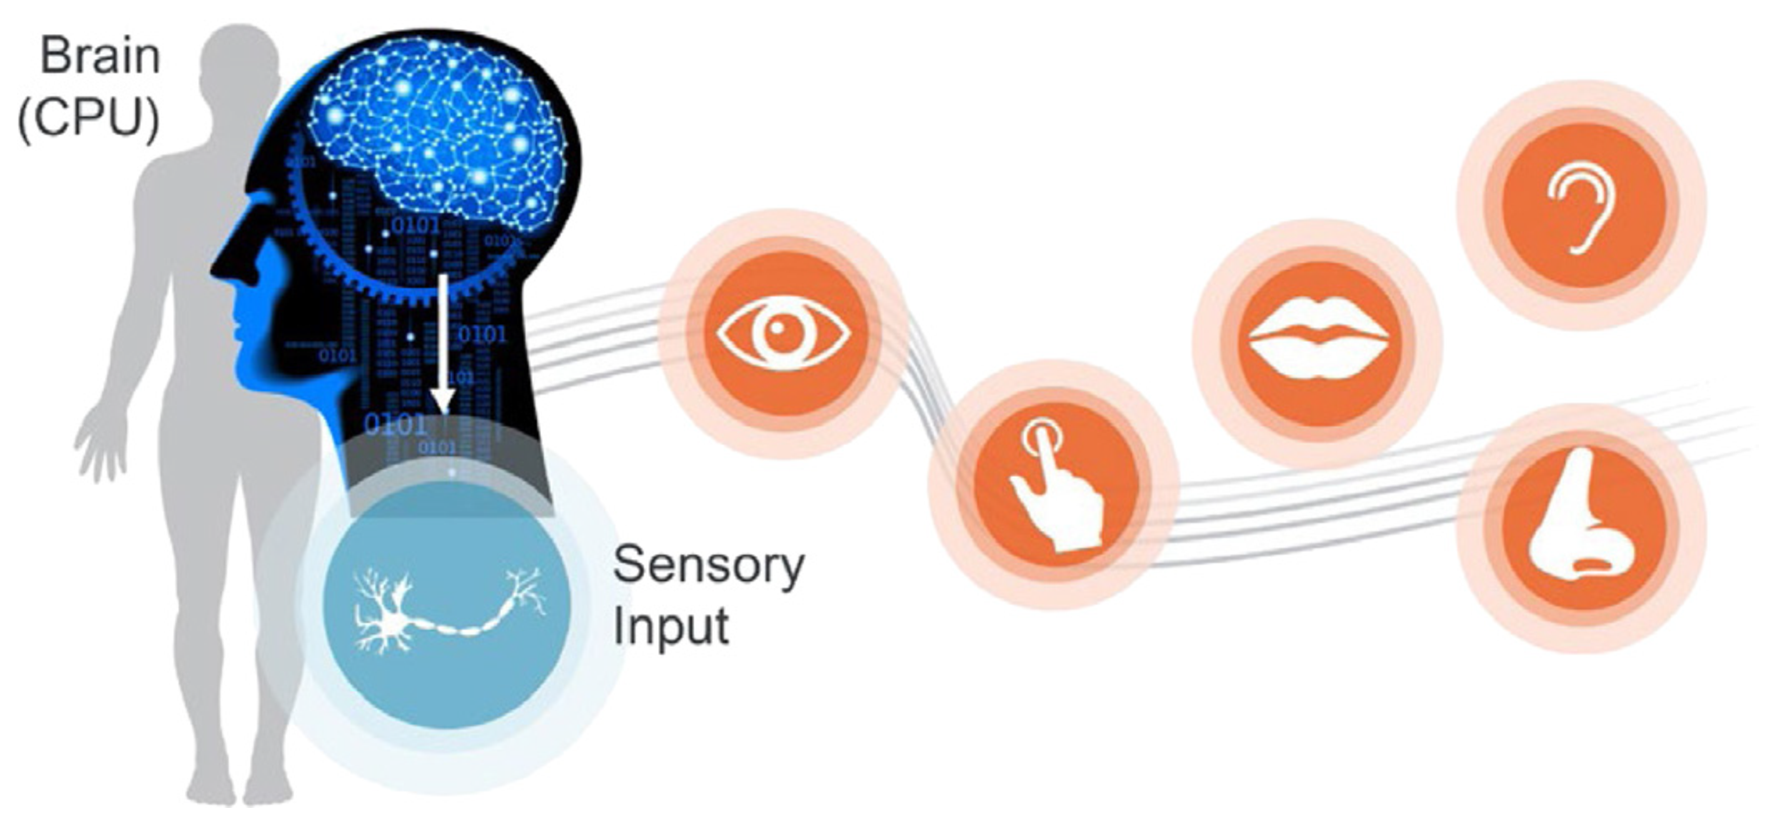
\includegraphics[width=10cm]{humanCommunication}
 \caption{In human communication the brain relies on several sources of sensory inputs,  such as visual, haptic, auditory, and  olfactory to validate events. By processing different sources of information consciously and unconsciously incomplete information can be compensated. Image from \cite{Poria2017}.}
 \label{fig:humanCommunication}
 \end{figure} 

Nevertheless, pathologies exist which hinder the proper encoding or decoding of communicated information. Some disorders which cause difficulties in communicating are autism, brain tumours, dementia (ex. \gls{ad}), \gls{pd}, \gls{hd}, \gls{ms}, and Epilepsy. All voice, language, speech, and swallowing problems make part of communication disorders and can be classified into speech and language disorders (more information in chapter~\ref{sec:SLP}). 

In \cite{Ruben2000}, Robert Ruben predicts that communication disorders will be a major public health challenge for the 21st century. According to Ruben, the economic basis of American society has undergone fundamental changes. In the beginning of the last century, at least 80\% of the American labor force were employed in tasks that depended on manual habilities. However, at the end of the same century already 62\% of the American labor force work in jobs using skills based on their communication abilities and of the remaining 37\% which are defined as farming and blue collar, many are also dependent on their communication abilities, as farmers have become farm managers. In this scenario, communication disorders present a great disadvantage. It has been estimated that communication disorders have a prevalence of 5\% to 10\% and that people suffering from them are economically more disadvantaged than those with hearing loss or other disabilities. Kruse shows in \cite{Kruse1997} that people unable to hear are less unemployed (47.6\%) than people with difficulty in speaking understandably (67.6\%). Ruben concludes in \cite{Ruben2000} that communication disorders may cost the U.S. \$154-\$186 billion per year, which is equal to 2.5\%-3\% of the Gross National Product.

As the ability to communicate effectively became an integral part of the fitness of a person, it is essential to increase allocation of resources to optimize the communication abilities of society as well as to invest in prevention and early detection of communication disorders. Prevention, diagnosis, and therapy of speech and language disorders are part of a SLP's job. In the following, speech and language pathologies will be presented as well as tools that \glsplural{slp} use to perform their job.

% ==================================================================
\section{Speech and Language Disorders}
\label{sec:SLP}

\theoremstyle{definition}
\begin{definition}{Speech-language pathology\\}
Speech-language pathology services are those services necessary for the \textbf{diagnosis} and \textbf{treatment} of swallowing (\gls{dysphagia}), speech-language, and cognitive-communication disorders that result in communication disabilities. Speech-language pathologists treat disorders of speech sound production (e.g., articulation, \gls{apraxia}, \gls{dysarthria}), resonance (e.g., hypernasality, hyponasality), voice (e.g., phonation quality, pitch, respiration), fluency (e.g., stuttering), language (e.g., comprehension, expression, pragmatics, semantics, syntax), cognition (e.g., attention, memory, problem solving, executive functioning), and feeding and swallowing (e.g., oral, pharyngeal, and esophageal stages). (Page 4 in \cite{SLPathologies})
\label{def:SLP}
\end{definition}

\glsplural{slp} diagnose and treat patients with voice, speech, language, and swallowing disorders (see above Def.\ref{def:SLP}). Communication disorders can be found in all age groups. It is estimated that 40 million Americans have communication disorders. In the following some detailed facts are listed \cite{SLPathologies}:

\begin{itemize}
\item 6-8 million people in the United States (US) have some form of language impairment.
\item Roughly 1 million people in the US suffer from aphasia. 
\item More than 3 million Americans stutter. 
\item About 5\% of children have noticeable speech disorders by the first grade 
\item Specific language impairment is one of the most common childhood disorders, affecting 7\%-8\% of children in kindergarten. 
\item Approximately 7.5 million Americans have trouble using their voices.
\item 1 million people in the US currently suffer from \gls{pd}, with an estimated 50,000-60,000 new cases diagnosed annually. 
\item It is estimated that 89\% of individuals with \gls{pd} worldwide have a speech or voice disorder, but only 3\% to 4\% receive speech or voice treatment. 
\item An estimated 300,000-600,000 people per year are affected by \gls{dysphagia} resulting from neurologic disorders. 
\item Each year an estimated 2.4 million individuals in the U.S. sustain a \gls{tbi} and another 795,000 individuals sustain an acquired brain injury (ABI) from nontraumatic causes.
\end{itemize}

The listed communication disorders can have different etiologies. Communication disorders can be caused by neonatal problems (e.g., prematurity, low birth weight, substance exposure) or developmental disabilities (e.g., specific language impairment, autism spectrum disorder, dyslexia, attention deficit/hyperactive disorder). Also oral anomalies (e.g., cleft lip/palate, dental malocclusion, macroglossia, oral-motor dysfunction) and neurological diseases/dysfunctions (e.g., \gls{tbi}, \gls{cp}, cerebral vascular accident, dementia, \gls{pd}, \gls{als}) can cause several communication problems.

Especially progressive neurological diseases and disorders of the brain can have a huge impact on communication abilities. \gls{ad} is one of the most common forms of dementia and its progression is approximately 10 years. This disease mainly affects people after the age of 60 and is usually diagnosed when two or more functions are affected, e.g. cognition and language which are the first to impaired. Communication problems that are associated with \gls{ad} are \gls{apraxia} of speech, \gls{dysarthria} (most commonly hypokinetic dysarthria) \todo{include definition in glossary} and word finding difficulties. The expressive language skill maybe intact, but their verbalisations become confused or out of context and with the progression of the disease their understanding becomes poorer and some patients even become speechless or unresponsive. Some patients with \gls{ad} also become emotional or particularly depressed. \cite{communicationDifficulties} 
 
\gls{pd} is also a progressive neurological disease which has increased in incidence, as did longevity. First symptoms include disordered speech and swallowing difficulties and usually appear after the age of 50. A common speech problem is \gls{dysarthria} which may be caused by a combination of problems with respiration, phonation, resonance, prosody, and articulation. All of these factors result in a decerase in intelligibility. Dysphonia may occur which leads to a weak voice. For patients it can be difficult to finish sentences and due to changes in manner and place of articulation the articulation of consonants can become disordered. Some people with \gls{pd} experience pailalia where words follow each other at a rapid speed and some phrases are repeated continuously. Speech may become monotonous and some patients experience difficulties with resonance, caused by a rigid palate and failure to close the nasopharynx leading to hyper nasality.\cite{communicationDifficulties}

Another neurological disease that can appear between the ages of 20 to 40 years is \gls{ms}. Severe symtpoms can follow this disease but the majority of patients with \gls{ms} continue to live active lives. However, around 50\% of \gls{ms} patients have speech difficulties, and \gls{dysarthria} is common. 
Problems with prosody, phonation and articulation can occur as well as harsh or breathy voice and difficulties with control of pitch, rate, and volume. It is estimated that around 50\% of people with \gls{ms} have difficulties with
articulation and 25\% have some form of hypernasality. Some strategies to improve communication following a diagnosis of \gls{ms} include breath exercises to improve volume and sentence length as well as speech muscle exercises to improve dyarthric speech. \cite{communicationDifficulties}




Stuttering: public stigma \cite{Boyle2016}.

relationship between the experience of stuttering and demographic characteristics of adults who stutter\cite{Freud2017}

Effects of Music therapy on stuttering \cite{Baumann2017}\\

Relationship of stutter severity and emotional stress \cite{Choi2016}, \cite{Smith2017}, \cite{Vanryckeghem2001}, \cite{Alm2015}\\




Questions from Stuttering Center Western Pennsylvania\\
- What makes a person stutter on a particular word or utterance?\\
- Which measures are most important when evaluating stuttering, and what is the most reliable way to obtain these measures?\\
- How do we document improvements in treatment when many of the changes are "under the surface" (e.g., changes in feelings or attitudes toward speaking)?\\
- How well does treatment work, and how does a clinician determine what type of treatment is best for a specific individual who stutters?\\
"Many current treatments for stuttering in school-age children, adolescents, and adults are based on finding a balance between helping speakers improve their fluency through changes to speech production ("speech modification" techniques) and helping speakers improve their attitudes and feelings about stuttering to reduce the severity of stuttering ("stuttering modification" techniques). Ultimately, the goal of treatment is to reduce the overall impact of stuttering on the person's life."\\

 
Stuttering treatment: brain research \cite{Ingham2017}\\

Video self-modeling as a post-treatment fluency recovery strategy for adults\cite{Harasym2015}\\

\begin{comment} 
\section{Diagnosis and Therapy of Speech and Language Pathologies}

The American Speech-Language-Hearing Association (ASHA) defines that all individuals of all ages are eligible for speech-language pathology services if their ability to communicate and/or swallow effectively is reduced or impaired. Also if there are risk factors which lead to believe that treatment would prevent development of a speech, language, communication, or feeding and swallowing disorder; reduce the degree of impairment; lead to improved functional communication skills and/or functional feeding and swallowing abilities; or prevent the decline of communication and/or swallowing abilities. The referral can happen by the individual, family members, audiologists, physicians or teachers. \cite{SLPathologies}

Types of documentation: assessment documentation, treatment documentation, daily notes, progress reports. (SLP Manual page 6)

Medicare classifies therapy as rehabilitative or maintainance programs. (SLP Manual page 9)

\url{http://www.asha.org/MapLanding.aspx?id=8589947062} evidence maps which shows you recent articles and their conclusions. Shows also patients view.

patients with dementia like talking mats.

Screening of dementia in low-literate settings: The following instruments were validated in a low-literate or illiterate setting: Mini Mental State Examination (MMSE), Cognitive Abilities Screening Instrument (CASI), Eurotest, and Fototest. "At present, although existing screening tools demonstrate reasonably good accuracy in low-literacy settings, the available evidence is inadequate to allow recommendation of any one particular test" (p. 30). Further research is needed for measures designed for populations with low literacy, and those living in low- and middle-income countries. (Cognitive Screening Tools for Identification of Dementia... Paddick 2017)

Cognitive-Communication Treatment (Cognitive Deficits, Cognitive
Rehabilitation), Fluency Treatment (Stuttering, Cluttering), Language Treatment (Receptive, Expressive, Pragmatics or Social
Communication, Reading, Writing), Myofunctional Treatment (Tongue Thrust), \textbf{Neurological Motor-Speech Treatment}, \textbf{Social Communication Treatment} (Body language, facial expression, emotional
understanding, speech style, social reasoning, and making inferences are examples of elements of social communication.), Speech Sound Disorders Treatment (Articulation Disorder Treatment, Phonological Process Disorder Treatment), Swallowing Treatment (See also Dysphagia) is where mostly instruments are required(videofluoroscopy, endoscopy, ultrasound, manometry, electromyography, more on page 26), Voice and/or Resonance Treatment (also needs more instruments p. 28), 



%-----------------
SLPs have different devices they can use to diagnose or treat speech or language disorders. Besides using visual tools to work with children as seen in Fig.~\ref{fig:tools}~a) (more examples in \footnotemark) and mirrors for the patients to observe their own movements during speech exercises, they also use medical equipment for more comprehensive tests. In Fig.~\ref{fig:tools}~b) an electroglottograph (EGG) \todo{in glossary} also called laryngograph is shown which is employed to measure non-invasively the degree of contact between vibrating vocal folds during voice production. It has been applied to patients with hear loss and dysphonia.

electropalatography

airflow machine

ultrasound

\footnotetext{\url{http://www.mnsu.edu/comdis/kuster2/sptherapy.html}}
https://www.speechbuddy.com/parents/how-it-works/products/speech-buddies-set


visual feedback tool is important as audio feedback is not useful as they have been doing the sounds and for them it is correct. it is not a guesswork anymore, not the patietns opinion or the therapists opinion. Children love technology. it is like a game, they can compete against therapist and are motivated to improve. also valuable for therapists as they can better explain to students how to produce sounds. apraxia, residual articulation problems where traditional therapy didn't help. 
http://completespeech.com/smartpalate/

sound measuring apparatus/ decibel meter: electroglottograph (EGG), laryngograph

stroboscopes: diagnostic stroboscopes, video stroboscopes

tablet computer: tablets are engaging, portable, affordable, multifunctional, apps designed for \gls{slp}

AAC, or augmentative and alternative communication, is a series of interventions used to help children with severe communication disorders communicate. Many apps are designed based on this method of therapy.

Analytical Software:
Language Analysis Software,
Signal Analysis Software,
Speech Analysis Software

Medical Software:
Aphasia Treatment – Aphasia Tutor by Bungalow Software,
Multi-Speech - KayPENTAX,
Speech Training System – Video Voice,
Text to Speech – Universal Reader by Premiere Assistive Technology

\begin{figure}[htbp]
\centering
 \subbottom[Example of games that can be used for SLP therapy.Descriptive game from ]{%
    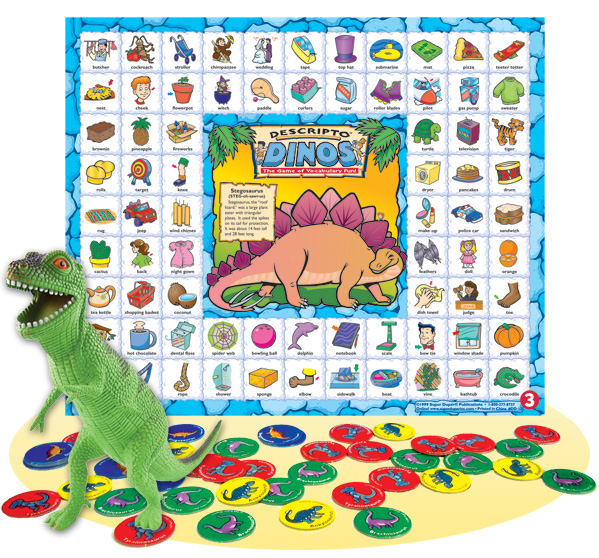
\includegraphics[width=0.4\linewidth]{gameSLP}}%
 \subbottom[Electrglottograph also called laryngograph]{%
    \hspace{0.5cm}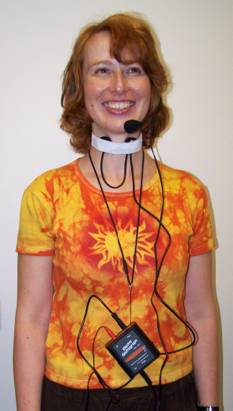
\includegraphics[width=0.4\linewidth]{egg}}
 \subbottom[Airflow machine]{%
    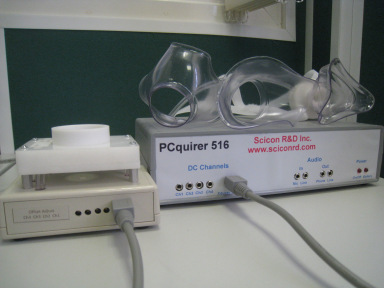
\includegraphics[width=0.4\linewidth]{airflow_machine}}%
    \subbottom[ultrasound]{%
    \hspace{0.5cm}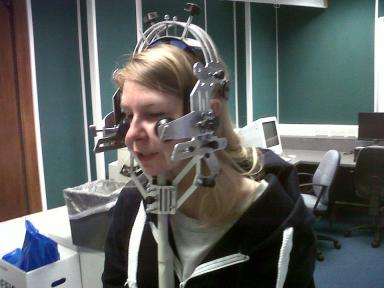
\includegraphics[width=0.4\linewidth]{ultrasoundhat}} 
 \subbottom[Palatometer with electrodes]{%
    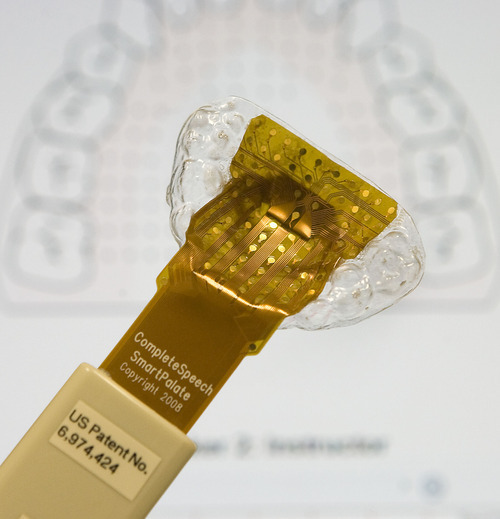
\includegraphics[width=0.4\linewidth]{palatometer}}    	
\subbottom[Smart palate]{%
    \hspace{0.5cm}\includegraphics[width=0.4\linewidth]{smartpalate}}%
 
\caption{Devices used by SLPs}
\label{fig:tools}
\end{figure}


%\footnotetext{\url{https://www.superduperinc.com/}}
%\footnotetext{\url{https://phonlabmanchester.wordpress.com/resources/}}



\end{comment}

% ==================================================================


\section{Speech Production Anatomy}
For verbal communication besides tongue, larynx, pharynx, and soft palate muscles, which are not visible from the exterior, also lip and mandibular muscles are crucial (orbicularis oris: close lips, levator labii superioris: raise upper lip, more in \cite{PhonManual}). 
Malfunction of these muscles can be caused by neurological or motoric problems, causing f.ex. speech disorders or facial paralysis. 

\begin{figure}
    \centering
    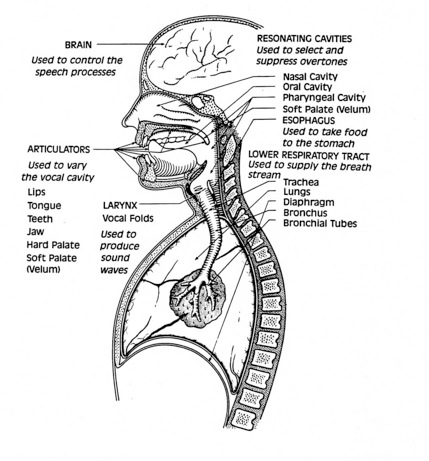
\includegraphics[width=10cm]{Anatomy-of-Speech-Graphic}
    \caption{Speech production Anatomy.}
    \label{fig:speechmuscles}
\end{figure}


% ==================================================================

\section{Facial Muscles}
\label{sec:anatomy}

The human face is composed by 43 muscles. Without them we would be missing an important tool for communicating not only with people from our cultural environment but also with people from different provenience as the only way to be understood would be through gestures. Our facial muscles are essential for both, verbal and non-verbal communication.\par 

The muscles of facial expression are thin, flat muscles that act either as sphincters of facial orifices, as dilators, or as elevators and depressors of the eyebrows and mouth. Frontalis, corrugator supercilii, depressor supercilii, procerus, and orbicularis oculi represent the periorbital facial muscles. The perioral muscles include the levator muscles, zygomaticus major and minor, risorius, orbicularis oris, depressor anguli oris, depressor labii, and mentalis. The nasal group includes compressor naris, dilator naris, and depressor septi. In the neck, the platysma muscle lies superfi cially and extends into the lower face (see Fig.~\ref{fig:facemuscles}).\cite{Prendergast2013anatomy}


\begin{figure}
    \centering
    \includegraphics[width=10cm]{face_muscles}
    \caption{Muscle anatomy of the human face (anterior view).\cite{Prendergast2013anatomy}}
    \label{fig:facemuscles}
\end{figure}


\begin{comment}
% ==================================================================
\section{Automatic Facial Expression Recognition}
\label{sec:compRepresentation}
\begin{figure}
{\footnotesize
\begin{forest}
    for tree={
      edge path={
        \noexpand\path [draw, thick, \forestoption{edge}] (!u.parent anchor) -- +(5pt,0) |- (.child anchor)\forestoption{edge label};
      },
      parent anchor=east,
      child anchor=west,
      grow'=east,
      text centered,
      minimum width=1in,
      text width=2.4cm
      }
 [Automatic\\  Facial\\ Expression Recognition [Parametrization [Descriptive] [Judgement]] [Recognition [Face \\ localization [Detection] [Segmentation]] [Face \\ registration] [Feature \\ extraction [Predesigned [Appearance][Geometry][Appearance + Geometry]][Learned]] [Expression\\ Classification /Regression [Categorical] [Continuous]] [Multimodal \\fusion [Direct fusion][Early fusion][Late fusion] [Sequential]]]]
  \end{forest}
}
\caption{Taxonomy for AFER adapted from \cite{Corneanu2016survey}.}
\label{fig:AFER}
\end{figure}

Automatic Facial Expression Recognition (AFER) is an interdisciplinary domain in which researchers from behavioural science, neurology, psychology, and computer science investigate the recognition of facial expressions which can give us insights about the emotional state of a person.

\subsection{Parametrization of FEs}




\subsection{Recognition of FEs}

\subsubsection{Face Localization}

\subsubsection{Face Registration}

\subsubsection{Feature Extraction}

\subsubsection{FE Classification and Regression}

\subsubsection{Multimodal Fusion Techniques}

\subsection{3D representations}
\cite{Sandbach2012survey}
\subsection{Thermal}


\end{comment}


% ==================================================================
\begin{comment}
\section{Example glossary and acronyms}
%
% \todo[inline]{A a note in a line by itself.}
%
This is the first occurrence of an abbreviation: \gls{abbrev}.

And now the second occurrence of the same abbreviation: \gls{abbrev}.

And a new acronym with capital letter: \Gls{xpt} and reused \gls{xpt}.

Lets add the term ``\gls{computer}'' to the glossary!

\end{comment}